\documentclass[11pt]{article}
\usepackage{amsmath, amssymb, amsthm}
\usepackage{graphicx}
\usepackage{hyperref}
\usepackage{enumitem}

\newtheorem{theorem}{Theorem}
\newtheorem{lemma}[theorem]{Lemma}
\newtheorem{definition}[theorem]{Definition}

\title{A Brief Note on the Gaussian Integral}
\author{O.\ Maclaren}
\date{\today}

\begin{document}
\maketitle

\begin{abstract}
We derive the classical Gaussian integral using polar coordinates and sketch its connection to probability theory. A short numerical example illustrates the accuracy of finite truncation.
\end{abstract}

\section{Introduction}

The \textbf{Gaussian integral}
\begin{equation}\label{eq:gauss}
  I = \int_{-\infty}^{\infty} e^{-x^2}\, dx = \sqrt{\pi}
\end{equation}
appears throughout mathematics, physics, and statistics. Despite its elementary appearance, the integrand $e^{-x^2}$ has no closed-form antiderivative, so the result must be obtained by indirect means.

\section{Proof via polar coordinates}

\begin{theorem}\label{thm:main}
$\displaystyle \int_{-\infty}^{\infty} e^{-x^2}\, dx = \sqrt{\pi}$.
\end{theorem}

\begin{proof}
Consider the square of the integral:
\[
  I^2 = \left(\int_{-\infty}^{\infty} e^{-x^2}\, dx\right)
        \left(\int_{-\infty}^{\infty} e^{-y^2}\, dy\right)
      = \int_{-\infty}^{\infty}\int_{-\infty}^{\infty} e^{-(x^2+y^2)}\, dx\, dy.
\]
Switching to polar coordinates $x = r\cos\theta$, $y = r\sin\theta$:
\[
  I^2 = \int_0^{2\pi}\int_0^{\infty} e^{-r^2}\, r\, dr\, d\theta
      = 2\pi \cdot \frac{1}{2} = \pi.
\]
Since $I > 0$, we conclude $I = \sqrt{\pi}$.
\end{proof}

\section{Connection to the normal distribution}

\begin{definition}[Normal distribution]
A random variable $X \sim \mathcal{N}(\mu, \sigma^2)$ has probability density function
\begin{equation}\label{eq:normal}
  f(x) = \frac{1}{\sigma\sqrt{2\pi}}\, \exp\!\left(-\frac{(x-\mu)^2}{2\sigma^2}\right).
\end{equation}
\end{definition}

The normalisation constant $\frac{1}{\sigma\sqrt{2\pi}}$ follows directly from~\eqref{eq:gauss} via the substitution $u = (x - \mu)/(\sigma\sqrt{2})$.

\begin{lemma}
For any $\sigma > 0$,
\[
  \int_{-\infty}^{\infty} \exp\!\left(-\frac{x^2}{2\sigma^2}\right) dx = \sigma\sqrt{2\pi}.
\]
\end{lemma}

\section{Numerical illustration}

Truncating the integral to a finite interval $[-a, a]$ converges rapidly:

\begin{center}
\begin{tabular}{rcc}
\hline
$a$ & $\displaystyle\int_{-a}^{a} e^{-x^2}\, dx$ & Relative error \\
\hline
1 & 1.4936 & 15.7\% \\
2 & 1.7642 & 0.39\% \\
3 & 1.7724 & $4.2 \times 10^{-5}$ \\
4 & 1.7725 & $< 10^{-8}$ \\
\hline
\end{tabular}
\end{center}

The decay of $e^{-x^2}$ is so rapid that even $a = 3$ captures the integral to five significant figures.

\section{The Gaussian in higher dimensions}

The result generalises to $\mathbb{R}^n$. For a symmetric positive-definite matrix $\Sigma \in \mathbb{R}^{n \times n}$:
\begin{equation}\label{eq:multivariate}
  \int_{\mathbb{R}^n} \exp\!\left(-\tfrac{1}{2}\, \mathbf{x}^\top \Sigma^{-1} \mathbf{x}\right) d\mathbf{x}
  = \sqrt{(2\pi)^n \det \Sigma}.
\end{equation}

Key applications include:
\begin{enumerate}[label=(\roman*)]
  \item \textbf{Statistical mechanics} --- partition functions for harmonic systems
  \item \textbf{Quantum field theory} --- path integrals in free-field theories
  \item \textbf{Machine learning} --- marginalisation in Gaussian processes
  \item \textbf{Finance} --- Black--Scholes option pricing
\end{enumerate}

\section{A figure}

Figure~\ref{fig:gaussian} shows the Gaussian bell curve $e^{-x^2}$ with the area under the curve shaded.

\begin{figure}[h]
  \centering
  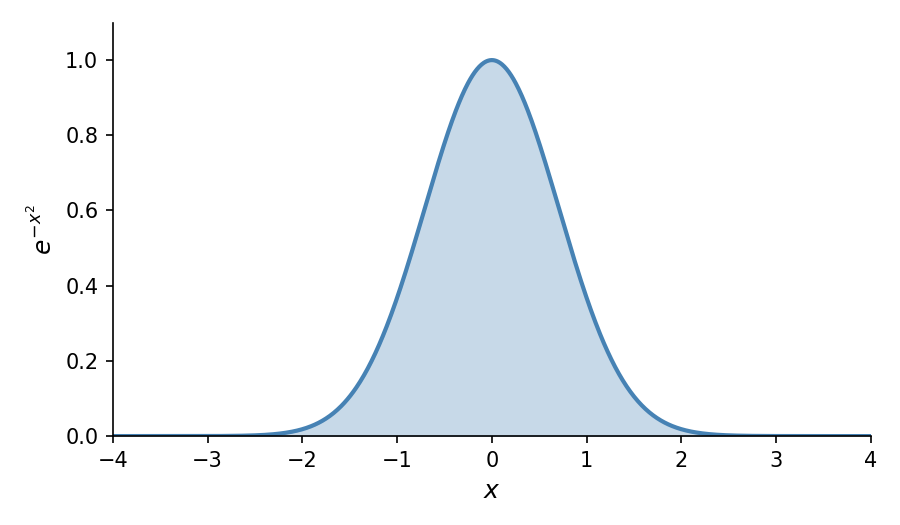
\includegraphics[width=0.6\textwidth]{gaussian_plot.png}
  \caption{The function $e^{-x^2}$ and its integral $\sqrt{\pi} \approx 1.7725$. The shaded region represents the total area under the curve.}
  \label{fig:gaussian}
\end{figure}

\section*{Acknowledgements}

This note was prepared as a test document for the \texttt{pi-markdown-preview} LaTeX rendering pipeline.

\begin{thebibliography}{9}
\bibitem{boros2004} G.~Boros and V.~H.~Moll, \emph{Irresistible Integrals: Symbolics, Analysis and Experiments in the Evaluation of Integrals}, Cambridge University Press, 2004.
\bibitem{conrad2013} K.~Conrad, ``The Gaussian integral,'' expository note, University of Connecticut, 2013.
\end{thebibliography}

\end{document}
